\chapter{Background}
\label{chp:chapter_2}

In this chapter the necessary background information will be covered to be able to fully understand the architecture of the proposed solutions, as well as defining useful terms. 

\section{Wireless Connection}
\label{sec:ch2_wireless_connection}
A wireless connection is setup between at least two devices. Within the bluetooth low-energy specification there exists a clear hierarchy, where one device is dominent and is called the Central. The central usually takes the shape of a phone or a laptop. The other side of the connection is with one or more Peripherals. These devices include headphones, smartwatches, IoT sensors, pushbuttons and much more. 

For the sake of this thesis I define three phases for a BLE connection. These phases are:
\begin{itemize}
    \item \textit{Unconnected}: before any connection is established between the Central and the Peripheral
    \item \textit{Connecting} or \textit{Connection Setup}: starts from the connection request and ends when the last non-application packet is sent. 
    \item \textit{Connected} or \textit{Application}: starts when connection setup is finished and only application packets are sent. Application packets are packets that are necessary to fullfil the application. 
\end{itemize}
These terms are not officially defined by the BLE specification, but are used throughout the thesis. 

\section{Advertisers and Scanners}
When in an unconnected state, the Peripheral and Central can take on the roles of \textit{Advertiser} and \textit{Scanner} respectively. As an Advertiser, a Peripheral sends out advertising packets. Advertising packets can contain up to 31 bytes of advertising data. The structure of the advertising data is shown in Figure \ref{fig:advdata_layout}. The \texttt{AD Type} field is an 8 bit identifier which refers to one of the many predefined advertisement datatypes. This is followed by the length of the data for this type and then the actual data. 

\begin{figure}[]
    \centering
    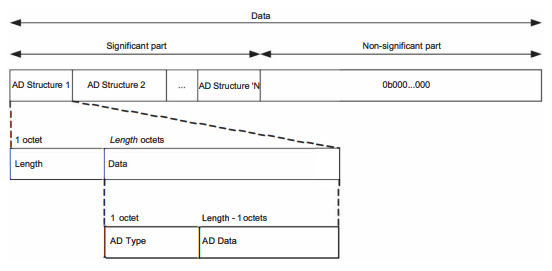
\includegraphics[width=0.8\textwidth,height=6cm,keepaspectratio=true]{images/advertising_data}
    \caption{
        Layout of the AdvData field for advertisement packets as per the bluetooth core specification \cite{bluetooth_spec}.
    }
    \label{fig:advdata_layout}
\end{figure}

There are multiple different advertising modes, but the only one used in this thesis is the \texttt{ADV\_IND}. This mode has two traits which are \textbf{Connectable} and \textbf{Scannable}. Connectable means that the Peripheral is open for connection requests. Scannable means that a Central can, as a response to an advertising packet, send a \textit{Scan Request} to request more data from the Perihperal. This data is then sent in the form of a \textit{Scan Response} and allows for another 31 bytes of advertising data.

\section{Connection Parameters}
The connection setup is initiated by the Central by responding with a \texttt{CONNECT\_IND} packet to an advertisement packet. From this moment a connection between the devices is made and the setup can begin. The parameters which decide the connection configuration are contained within the \texttt{LLData} field of the \texttt{CONNECT\_IND} packet. The most important configuration values to understand are \textit{Connection Interval} (CI) and \textit{Peripheral Latency} (PL). 

\begin{figure}[]
    \centering
    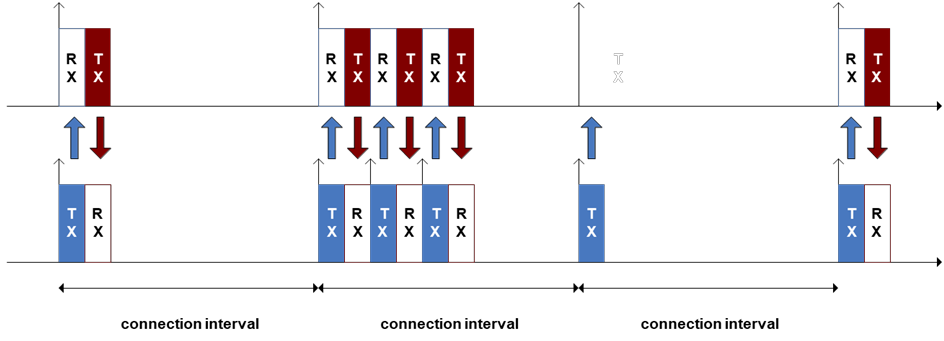
\includegraphics[width=0.8\textwidth,height=6cm,keepaspectratio=true]{images/connection_interval_slave_latency}
    \caption{
        \color{red} Red \color{black} is the Peripheral and \color{blue} blue \color{black} is the Central. From Nordic Semiconductors \cite{nordic_2022}.
    }
    \label{fig:ci_and_pl}
\end{figure}

As you can see in Figure \ref{fig:ci_and_pl}, the Connection Interval is the time between the start of chains of transmit (TX) and receive (RX) events. Multiple TX/RX events can happen within one chain, but when there is no more data to be sent then the current chain is over and new data can be transmitted at the following interval. Peripheral Latency defines how many Connection Intervals the Peripheral is allowed to skip. For example, take a CI of 2 seconds and a PL of 0, this means that every two seconds the Central transmits a packet and the Peripheral replies. Now take a CI of 2 and a PL of 1, in this case the Central transmits every two seconds, but the Peripheral is allowed to sleep every other packet, effectively making the time inbetween transmissions four seconds. 

\section{Services and Characteristics}
\begin{figure}[]
    \centering
    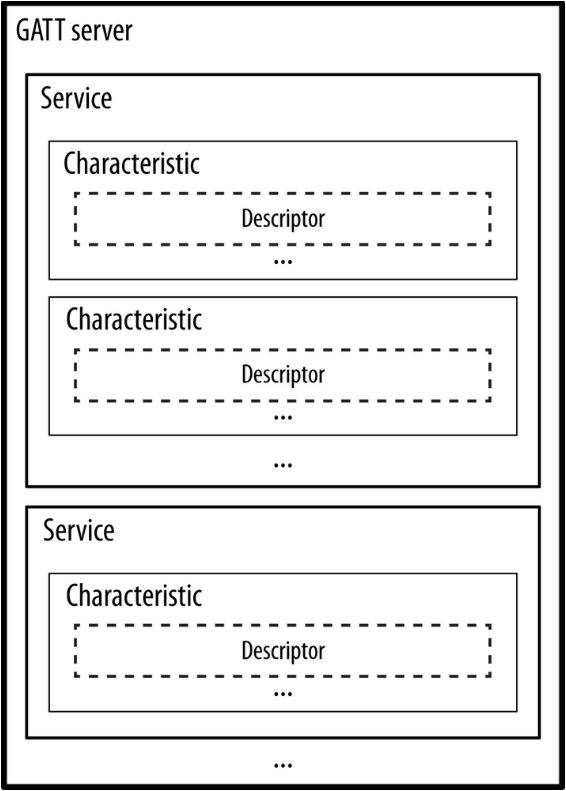
\includegraphics[width=0.5\textwidth,height=6cm,keepaspectratio=true]{images/gatt_service}
    \caption{
        Architecture of the GATT Server \cite{townsend_cufi}.
    }
    \label{fig:gatt_server}
\end{figure}
The \textit{Generic Attribute Profile} (GATT) defines how profile and user data is exchanged over a BLE connection. GATT defines the GATT Server, within which functionality is split up into \textit{Services}. Services contain datapoints called \textit{Characteristics}. These characteristics can be interpreted and configured using fields called \textit{Descriptors}. See Figure \ref{fig:gatt_server} for a schematic layout of the GATT Server.

\begin{figure}[]
    \centering
    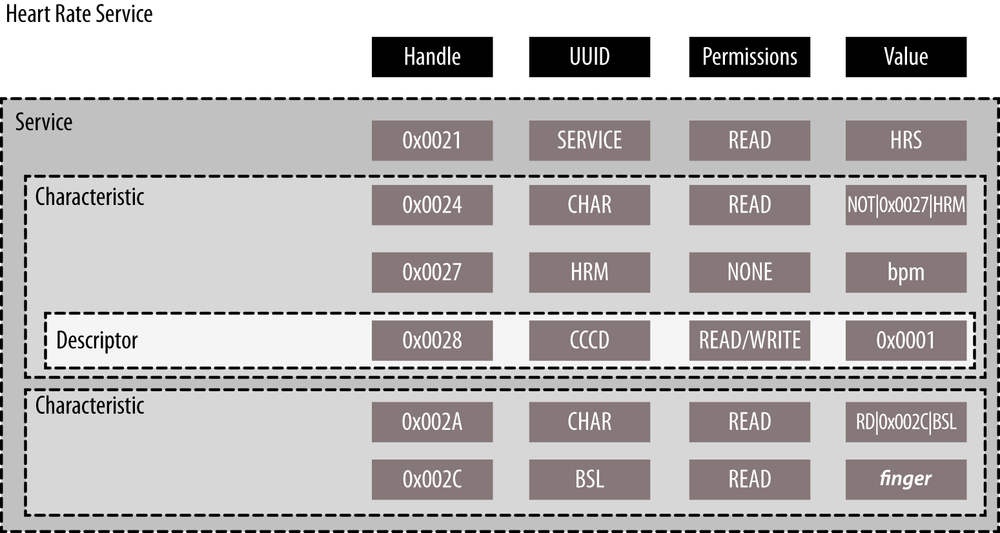
\includegraphics[width=0.5\textwidth,height=6cm,keepaspectratio=true]{images/heartrate_service}
    \caption{
        Heart Rate Service \cite{townsend_cufi}.
    }
    \label{fig:hrs_layout}
\end{figure}
To give a real world example, take the Heart Rate Service in Figure \ref{fig:hrs_layout}. This service allows a Client to read the heartrate sensor of a device. The heartrate service contains a characteristic called Heartrate. One of the descriptors tells us that the unit is defined as \textbf{beats per minute}. We could read the characteristic value manually, but if we would like to be notified when a new measurement is done then we can set the Notify bit of the \textit{Client Characteristic Configuration} or CCC descriptor.

To be able to read or write to a Characteristic we need its handle. The handle is a number that is unique for a characteristic within a GATT Server. To find this handle we can perform a \textit{Find By Type Request} using its 16-bit Universally Unique Identifier (UUID). Bluetooth SIG has predefined UUIDs for many predefined Services. Each predefined Service has a specification which defines the shape of the service. This includes all the Characteristics, Descriptors and their respective UUIDs.

The process of finding all these handles is what is called \textit{Service Discovery}. The result of this process is a list of numbers that can be used to read and write to the server. After Service Discovery is done the GATT Servers need to be configured. This usually means writing to the CCC descriptor to setup notifications for the desired Characteristics. This process will henceforth be refered to as Configuration. 

Both the Central and the Peripheral can be Servers and Clients at the same time. For example; a phone can provide the central time for a smartwatch to display on the watchface, while the smartwatch measures the heartrate for the phone to display within a health application. This means that a Service Discovery and Configuration needs to be performed by both the Central and the Peripheral.

\section{Link Layer}
The Link Layer is the part of the Bluetooth stack which is tasked with managing the wireless link and actually sending data frames. The Link Layer sits inbetween the higher level protocols like GAP and GATT and the Physical Layer which actually controls the radio.
Procedures are defined within the Link Layer to make sure both the transmitting radio and receiving are configured correctly.

The \textit{Features Exchange} procedure is used to exchange which features are supported by both radios. These feature sets can vary widely between versions of Bluetooth and can have a large impact on performance. To guarantee that both sides of the link communicate in the same manner, these features are exchanged by the Link Layer at the start of each connection.

The size of the packets that can be received by a radio can also vary and is usually dependent on the available memory. To make sure the best throughput is achieved this needs to be communicated using the \textit{Data Length Exchange}. This exchanges the largest Air packet that each radio is able to receive at once.

\section{Connection Setup}
As previously defined in Section \ref{sec:ch2_wireless_connection}, the connection setup starts from the Connection Request and ends when the last non-application packet is sent. The packets that occur during Connection Setup can be divided into four groups which correspond to the subjects discussed in the previous sections.
\begin{itemize}
    \item Link Layer
    \item Service Discovery
    \item Configuration
    \item Application
\end{itemize} 
The order in which they occur are usually Service Discover, Configuration and then Application, with Link Layer communication starting parallel to the Service Discovery from the start.